\documentclass{standalone}
% font set
\usepackage{ctex}
\usepackage{fontspec}
\usepackage[T1]{fontenc}
\usepackage[sc]{mathpazo}
\usepackage{anyfontsize}
\setmainfont{Source Serif 4}
\setsansfont{Source Sans 3}
\setmonofont{Menlo}
\setCJKmainfont[BoldFont=黑体-简 中等,ItalicFont=楷体-简 常规体]{宋体-简 常规体}

% colors
\usepackage[dvipsnames]{xcolor}
\definecolor{pku-red}{RGB}{139,0,18}
\usepackage{colortbl}
\newcommand{\light}[1]{\textcolor{Orchid}{#1}}
\newcommand{\contrastlight}[1]{\textcolor{TealBlue}{#1}}

% plots
\usepackage{tikz}
\usepackage{tikz-cd}
\usetikzlibrary{arrows}
\usetikzlibrary{arrows.meta,positioning,calc,3d}
\usepackage{pgfplots}
\pgfplotsset{compat=newest}
\tikzset{
    punkt/.style={
        rectangle,
        rounded corners,
        draw=black, very thick,
        minimum height=2em,
        inner sep=6pt,
        text centered,
        fill=gray!30
    }
}

% math package
\let\Bbbk\relax
\usepackage{amsmath}
\usepackage{mathrsfs}
\usepackage{amssymb}
\usepackage{amsfonts}
\usepackage{stmaryrd}
\usepackage{latexsym}
\usepackage{extarrows}
\SetSymbolFont{stmry}{bold}{U}{stmry}{m}{n}

\begin{document}
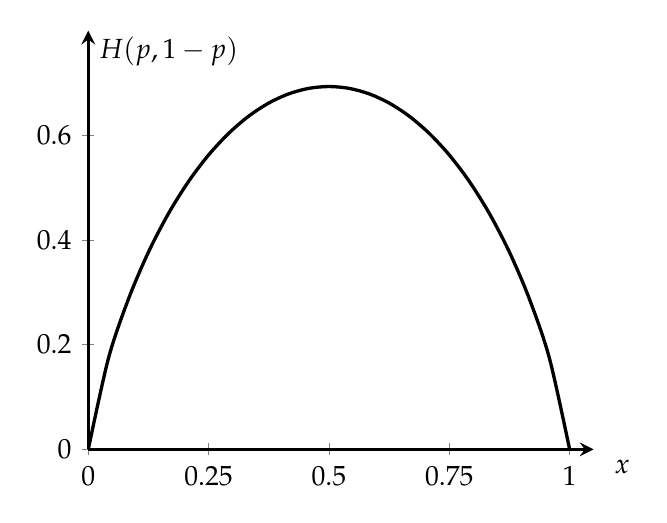
\begin{tikzpicture}
    \pgfplotsset{
    width=8cm,
    every axis/.append style={very thick},
    }
    \begin{axis}[
        ymin=0, ymax=0.8,
        xmin=0, xmax=1.05,
        axis x line=left,
        axis y line=left,
        legend style={draw=none},
        xtick={0,0.25,0.5,0.75,1},
        ytick={0,0.2,0.4,0.6},
        legend pos=south east,
        every axis x label/.style={
            at={(ticklabel* cs:1.02)},
            anchor=north west,
        },
        every axis y label/.style={
            at={(ticklabel* cs:0.95)},
            anchor=west,
        },
        label style={font=\normalfont},
        xlabel={$x$},ylabel={$H(p,1-p)$}
    ]
    \addplot[domain =0:1, smooth] {-x*ln(x)-(1-x)*ln(1-x)};
    \end{axis}
\end{tikzpicture}
\end{document}